\documentclass[12pt]{article}

\usepackage{adjustbox}
\usepackage{amsmath}
\usepackage[french, onelanguage]{algorithm2e}
\usepackage[french]{babel}
\usepackage[T1]{fontenc}
\usepackage{geometry}
\usepackage{glossaries}
\usepackage{graphicx}
\usepackage[hidelinks]{hyperref}
\usepackage[utf8]{inputenc}
\usepackage{listings}
\usepackage{lstautogobble}
\usepackage{tabularx}
\usepackage{textcase}
\usepackage{tikz}
\usepackage{tocloft}
\usepackage{verbatim}
\usepackage{xcolor}
\usepackage{fancyhdr}
\usepackage{fancyvrb}
\usepackage{microtype}
\usepackage{lmodern}
\usepackage{csquotes}
\usepackage{svg}
\usepackage{forest}
\usepackage{array}
\usepackage{pdflscape}
\usepackage{pdfpages}
\usepackage[
backend=biber,
style=numeric,
sorting=none
]{biblatex}
\addbibresource{valve.bib}
\DisableLigatures{encoding=*,family=*}
%\usepackage[pdf]{pstricks}
%\usepackage{auto-pst-pdf}
%\usepackage{uml}

\usetikzlibrary{shadows}

\newcolumntype{C}[1]{>{\centering}p{#1}}

\lstset{language=Java,
	keywordstyle=\color{RoyalBlue},
	basicstyle=\scriptsize\ttfamily,
	commentstyle=\ttfamily\itshape\color{darkgray},
	stringstyle=\ttfamily,
	breaklines=true,
	keepspaces=true,
	numbers=left,
	numbersep=5pt,
	showspaces=false,
	showstringspaces=false,
	showtabs=false,
	tabsize=4,
	autogobble=true,
	inputencoding=utf8,
	extendedchars=true,
	backgroundcolor=\color{gray!10},
	literate=
	{á}{{\'a}}1 {é}{{\'e}}1 {í}{{\'i}}1 {ó}{{\'o}}1 {ú}{{\'u}}1
	{Á}{{\'A}}1 {É}{{\'E}}1 {Í}{{\'I}}1 {Ó}{{\'O}}1 {Ú}{{\'U}}1
	{à}{{\`a}}1 {è}{{\`e}}1 {ì}{{\`i}}1 {ò}{{\`o}}1 {ù}{{\`u}}1
	{À}{{\`A}}1 {È}{{\'E}}1 {Ì}{{\`I}}1 {Ò}{{\`O}}1 {Ù}{{\`U}}1
	{ä}{{\"a}}1 {ë}{{\"e}}1 {ï}{{\"i}}1 {ö}{{\"o}}1 {ü}{{\"u}}1
	{Ä}{{\"A}}1 {Ë}{{\"E}}1 {Ï}{{\"I}}1 {Ö}{{\"O}}1 {Ü}{{\"U}}1
	{â}{{\^a}}1 {ê}{{\^e}}1 {î}{{\^i}}1 {ô}{{\^o}}1 {û}{{\^u}}1
	{Â}{{\^A}}1 {Ê}{{\^E}}1 {Î}{{\^I}}1 {Ô}{{\^O}}1 {Û}{{\^U}}1
	{ã}{{\~a}}1 {ẽ}{{\~e}}1 {ĩ}{{\~i}}1 {õ}{{\~o}}1 {ũ}{{\~u}}1
	{Ã}{{\~A}}1 {Ẽ}{{\~E}}1 {Ĩ}{{\~I}}1 {Õ}{{\~O}}1 {Ũ}{{\~U}}1
	{œ}{{\oe}}1 {Œ}{{\OE}}1 {æ}{{\ae}}1 {Æ}{{\AE}}1 {ß}{{\ss}}1
	{ű}{{\H{u}}}1 {Ű}{{\H{U}}}1 {ő}{{\H{o}}}1 {Ő}{{\H{O}}}1
	{ç}{{\c c}}1 {Ç}{{\c C}}1 {ø}{{\o}}1 {å}{{\r a}}1 {Å}{{\r A}}1
	{€}{{\euro}}1 {£}{{\pounds}}1 {«}{{\guillemotleft}}1
	{»}{{\guillemotright}}1 {ñ}{{\~n}}1 {Ñ}{{\~N}}1 {¿}{{?`}}1 {¡}{{!`}}1,
	texcl=true
}

\geometry{
	a4paper,
	total={170mm,237mm},
	left=20mm,
	top=30mm,
}

\pagestyle{fancy}
\setlength{\headheight}{56.4pt}
\addtolength{\topmargin}{-43.6pt}
\setlength{\footskip}{60pt}
\fancyhf{}
\rhead{
\includegraphics[width=4cm]{header.jpg}}
\rfoot{
\includegraphics[width=4cm]{footer.jpg}}

\title{Valve}
\author{Giorgio Caculli}
\date{\today}

\begin{document}
	\begin{titlepage}
		\centering
		\vspace*{\fill}
		\LARGE
		UE 209\\Organisation et gestion de l'entreprise
		\vspace*{\fill}
		\begin{center}
			\Large
			\textbf{Travail OGE\\}
			\Huge
			\textbf{L'entreprise Valve}\\
			\vspace*{0.5cm}
			\large
			\textit{Giorgio Caculli LA196672}
		\end{center}
		\vspace*{\fill}
		\begin{figure}[htbp]
			\centering
			\includesvg[width=\textwidth]{Valve_logo}
		\end{figure}
		\vspace*{\fill}
		\thispagestyle{fancy}
	\end{titlepage}

	\newpage
	\tableofcontents
	\thispagestyle{fancy}

	\newpage
	\section{Introduction}
	\textbf{Valve Corporation}, aussi connue sous le nom de \textbf{Valve Software}, est une entreprise américaine de développement et distribution de jeux vidéos située à Bellevue Washington \cite{wikipedia_valve}. Depuis sa fondation en 1996 par \textbf{Gabe Newell} et \textbf{Mark Harrington}, Valve a marqué son succès dans le monde vidéoludique grâce à ses célèbres titres et technologies:
    \begin{itemize}
        \item \textbf{Half-Life 2}
        \item \textbf{Counter-Strike}
        \item \textbf{Team Fortress}
        \item \textbf{Dota 2}
        \item Le \textbf{SteamVR}
        \item Les \textbf{Steam Machines}
    \end{itemize}
    Afin de permettre aux employés de choisir sur quels projets ils voudraient travailler, Valve a décidé de mettre en place une \textbf{structure hiérarchique horizontale} \cite{handbook}.

    \newpage
	\section{Structure de l'entreprise}
	Le site \textit{The Official Board} nous permet, dans un premier temps, de constater que l'entreprise suit une \textbf{structure \enquote{fonctionnelle}} \cite{theofficialboard}. Voici à quoi ressemblerait ce dernier:\\
	\begin{forest}
		for tree={
			if level=0{align=center}{% allow multi-line text and set alignment
				align={@{}C{25mm}@{}},
			},
			draw,
			font=\sffamily\bfseries,
			edge path={
				\noexpand\path [draw, \forestoption{edge}] (!u.parent anchor) -- +(0,-5mm) -| (.child anchor)\forestoption{edge label};
			},
			parent anchor=south,
			child anchor=north,
			l sep=10mm,
			s sep=19mm,
			tier/.wrap pgfmath arg={tier #1}{level()},
			edge={ultra thick, rounded corners=2pt},
			ultra thick,
			inner color=gray!5,
			outer color=gray!20,
			rounded corners=2pt,
			drop shadow,
		}
		[CEO\\Gabe Newell
			[COO\\Scott Lynch]
			[Art Director\\Jeremy Bennett]
			[Audio Director\\Tobin Buttram]
			[VP of Marketing\\Doug Lombardi]
		]
	\end{forest}\\
	Cependant, depuis que Valve décida de publier ses propres jeux, cette structure hiérarchique fut considérée comme \enquote{gênante}\cite{arstechnica}. Après avoir terminé de développer le jeu \textit{Half-Life 2}, une \textbf{structure horizontale} fut établie, cela signifie que les employés n'ont pas de directeur et ne sont pas le subordonné de quelqu'un \cite{handbook}.

	\begin{figure}[ht]
		\centering
		\includegraphics[page=13, width=\textwidth, angle=-90, clip, trim=15mm 10mm 15mm 5mm, scale=0.65]{hbook-FR.pdf}
		\caption{Diagrammes structurels de Valve (vu par les employés)}
		\label{fig:diag_valve_emp}
	\end{figure}

	\newpage
	\section{La fonction de direction}
    Selon sa structure horizontale, le principal acteur au niveau exécutif serait juste \textbf{Gabe Newell}, cependant, beaucoup d'autres experts entrent en jeu quand il faut faire des choix au niveau exécutif. Une longue liste du personnel est présente sur le site \textbf{\href{https://www.valvesoftware.com/en/people}{www.valvesoftware.com/en/people}}

    \section{Fonction de production}
    \subsection{Secteur économique: informatique}
    Depuis sa création, Valve corporation développe ses propres jeux vidéo ainsi que ses propres solutions hardware. On peut donc considérer que l'entreprise opère dans le \textbf{secteur secondaire}.\\
    Néanmoins Steam, la plateforme marketplace de Valve permettant d'acheter des jeux vidéo Valve, permet à des tiers de vendre leurs propres jeux. Jeux vidéo qui n'ont rien à avoir avec Valve, mais dont Valve récupère un pourcentage sur les ventes. On peut donc considérer que l'entreprise opère aussi dans le \textbf{secteur tertiaire}.

    \subsection{Processus de production}
    Comme cité dans le point précédent, étant donné que Valve produit et publie ses propres jeux vidéo, les mets à jour presque mensuellement, et développe même une suite à ses propres jeux vidéo, on pourrait considérer le processus de production chez Valve, comme étant une \textbf{production continue}.

	\section{La fonction marketing}

    \subsection{Public ciblé}
    Considérant la modernité des technologies développées et la focalisation vers le monde vidéoludique, nous pouvons supposer que Valve essaie de viser les joueurs et développeurs de jeux vidéo.

	\subsection{Part de marché}
    Quatre studios connus dans le monde vidéoludique sont affiliés à Valve, leurs fonctions diffèrent par rapport à leurs spécialisations, donc, voici les filiales et leurs fonctionnalités:
    \begin{itemize}
        \item \textbf{Turtle Rock Studios} - Développeur de jeux vidéos (2008) \cite{turtle_rock_studios}
        \item \textbf{Star Filled Studios} - Développeur de jeux vidéos (2012) \cite{star_filled_studios}
        \item \textbf{Impulsonic} - Son VR, son 3D et casque gaming (2017) \cite{impulsonic}
        \item \textbf{Campo Santo} - Développeur de jeux vidéos (2018) \cite{campo_santo}
    \end{itemize}

    \newpage
	\subsection{Principaux concurrents}
	Valve possède sa propre boutique en ligne où les utilisateurs peuvent acheter des jeux ou publier leurs propres jeux. Une boutique en ligne est une technologie utilisée pour vendre directement des produits (dans le cas de Valve ces sont digitalisés) à des clients. Ce genre de boutique n'est pas exclusif, et Valve doit faire face à beaucoup de concurrents, voici quelques uns des plus connus:
	\begin{itemize}
		\item \textbf{Epic Games Store} - Epic Games
		\item \textbf{Origin} - Electronic Arts
		\item \textbf{UPlay} - Ubisoft
		\item \textbf{Battle.net} - Blizzard
	\end{itemize}

    \subsection{La politique de place}
    La majorité des produits Valve peuvent être achetés via le marketplace \textbf{Steam}, nous pouvons déterminer que, à partir du moment où il y a aucun intermédiaire entre Valve et le client, le circuit mit en place par Valve serait un \textbf{circuit direct}.

    \subsection{La politique de prix}
    Valve, comme ses concurrents, suit deux types de tendances pour les prix des produits vendus sur ses plateformes. La première stratégie est de garder le même prix que les autres boutiques en ligne. Il y a donc \textbf{alignement des prix} avec le marché. Néanmoins, en période de vacances, Valve adopte une \textbf{stratégie de pénétration}. Cela signifie qu'une vaste quantité de produits est sujets à des réductions importantes \cite{valve_discout}.

	\newpage
	\subsection{Positionnement dans le marché}
	Le graphique ci-dessous nous montre le \textbf{nombre de joueurs total connectés en simultanés sur la plateforme Steam}. Le pic le plus élevé fut en \textbf{Mars 2021} qui compta \textbf{26.9 millions} d'utilisateurs. Voici le graphique représentant ces statistiques \cite{steamdb_user_count}:
    \begin{figure}[ht]
		\centering
		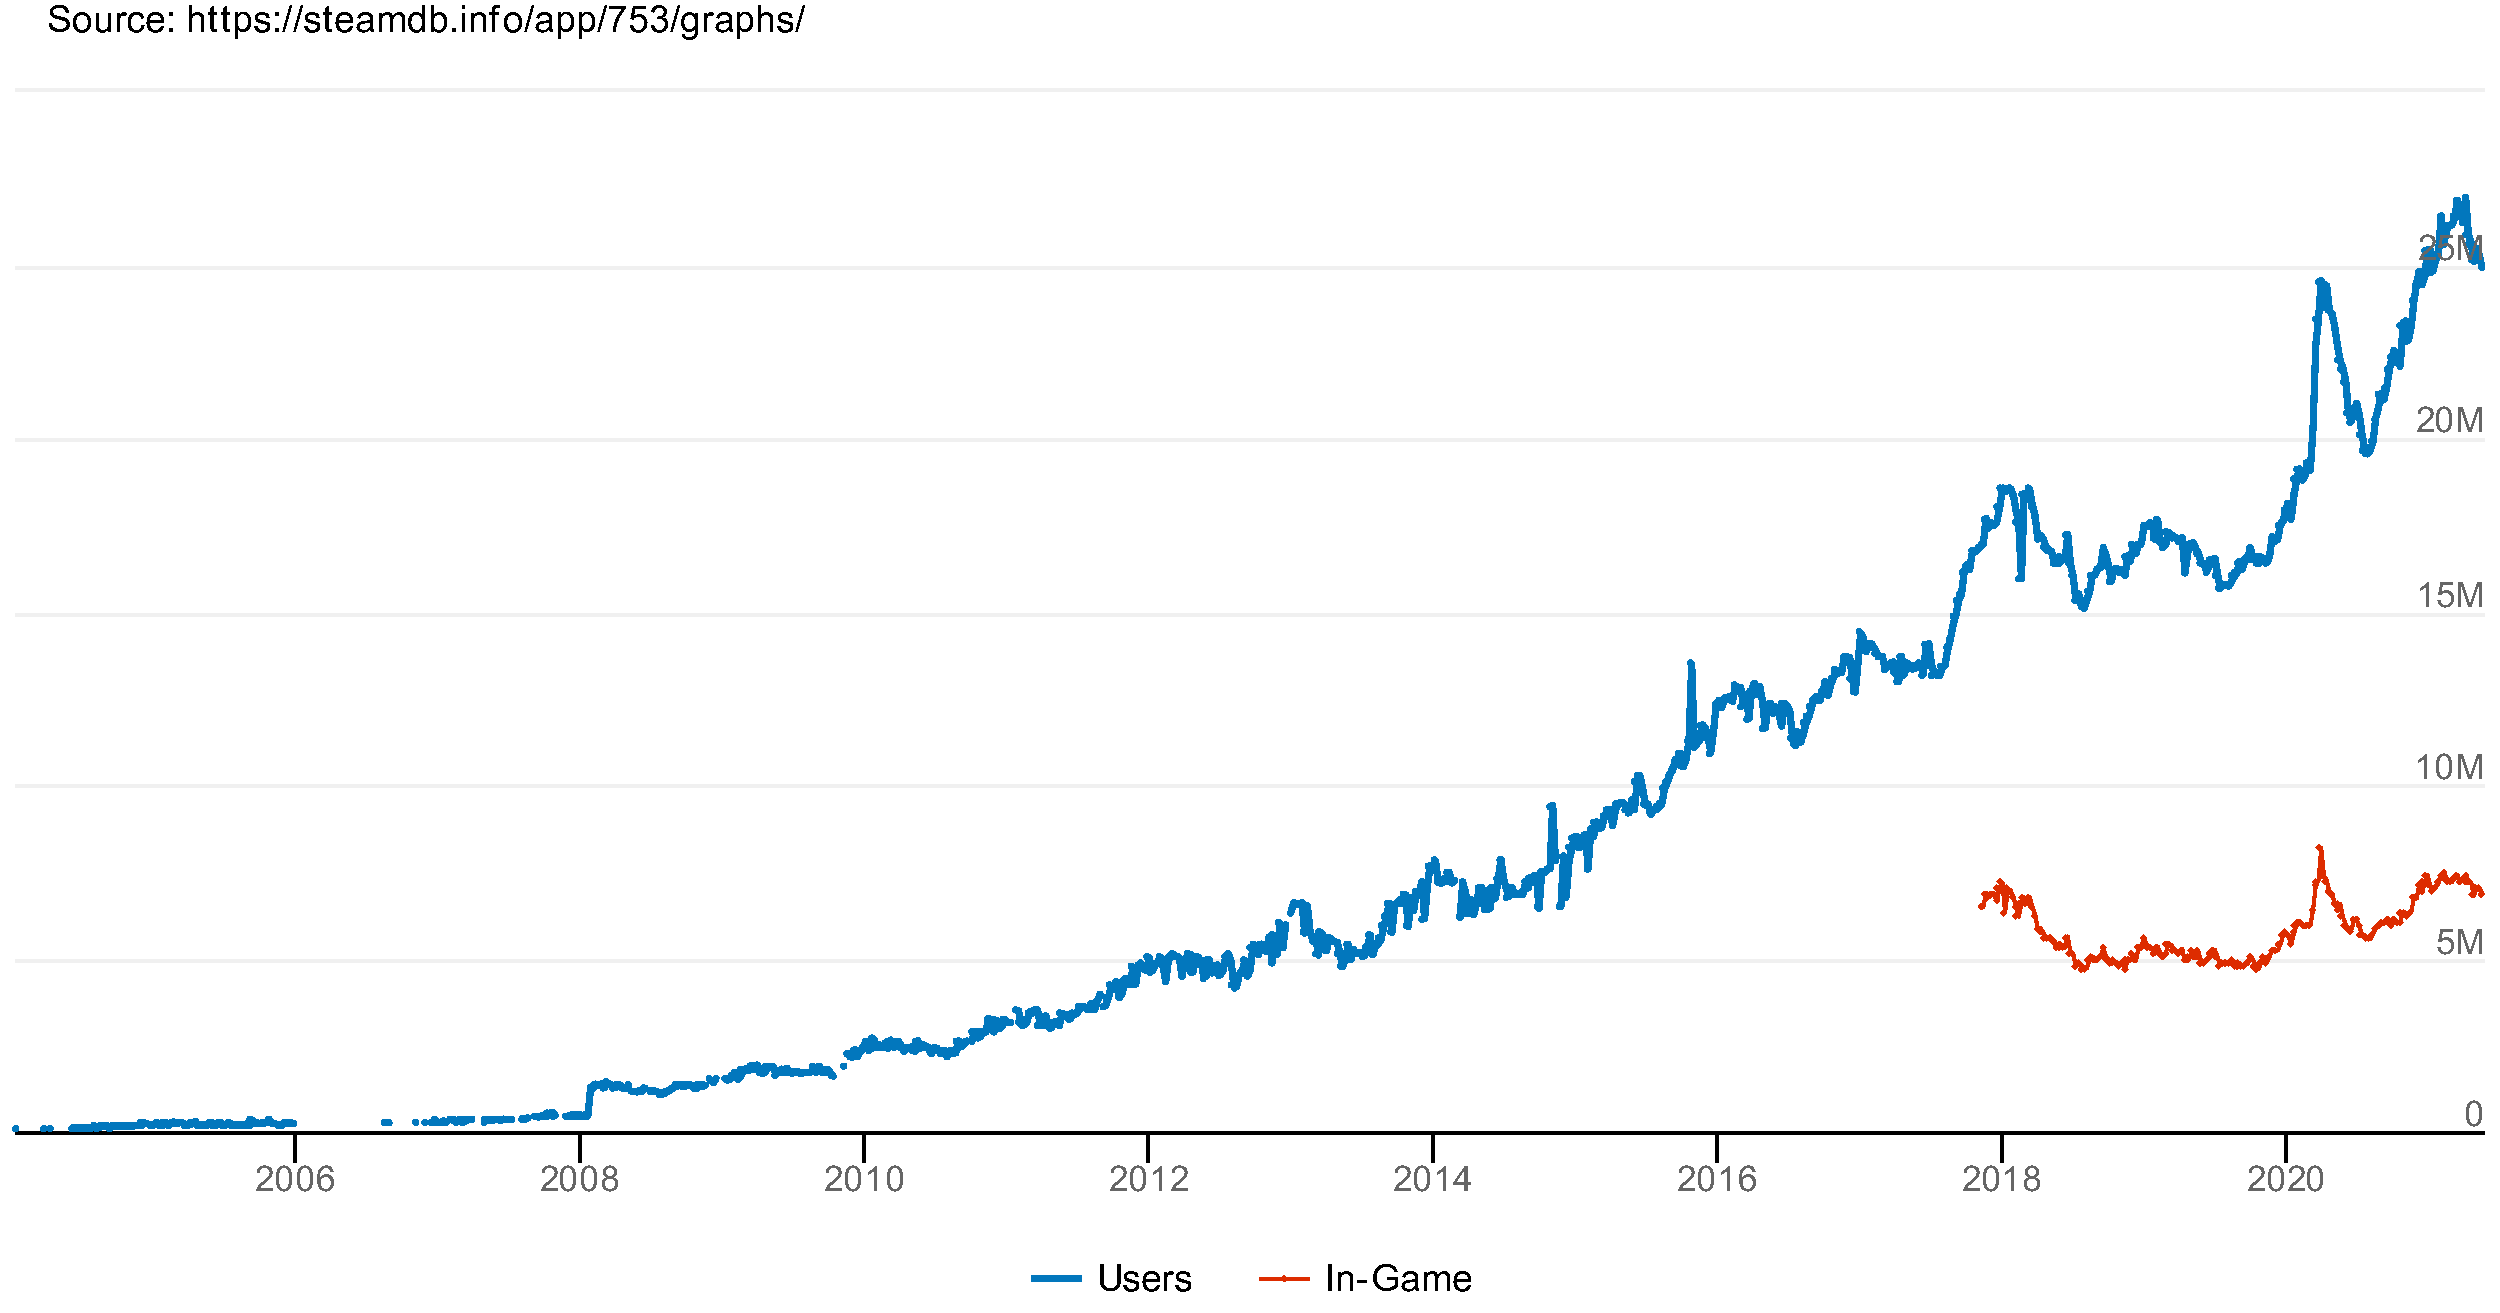
\includegraphics[page=1, width=\textwidth, angle=0, clip, trim=0mm 0mm 0mm 10mm, scale=1.0]{chart.pdf}
		\caption{Utilisateurs connectés en simultanés sur Steam}
		\label{fig:diag_steam_players}
	\end{figure}\\
	En contrepartie, le nombre de joueurs connectés en simultanés sur l'\textbf{Epic Games Store} fut de \textbf{13 millions en 2020} et \textbf{7 millions en 2019} \cite{epicgames_user_count} \cite{backlink_epic_user_count}. La différence entre joueurs connectés sur Steam en simultanés et joueurs connectés sur l'Epic Games Store en simultanés est de presque \textbf{206.9 \%}. Donc, le nombre de joueurs connectés sur Steam serait le double du nombre de joueurs connectés sur l'\textbf{Epic Games Store}.
    \begin{figure}[ht]
        \centering
        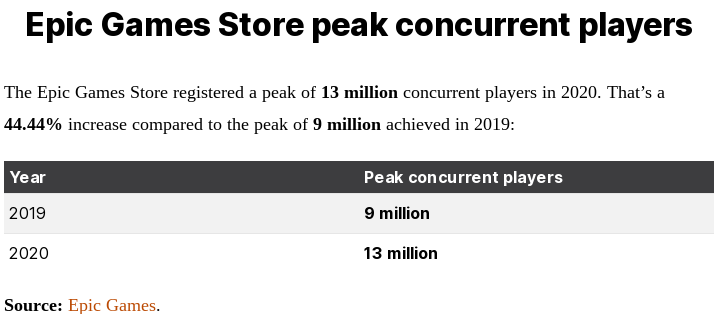
\includegraphics[clip, trim=0mm 0mm 0mm 0mm, width=0.8\textwidth]{player_count_epic.png}
        \caption{Utilisateurs connectés en simultané sur l'Epic Games Store}
    \end{figure}

	\newpage
	\section{Fonction R \& D}
	Valve a produit une vaste gamme de produits utilisés dans le monde vidéoludique, les principales technologies plus célèbres qui sont toujours en phase de développement sont:
	\begin{enumerate}
		\item \textbf{Proton} - technologie permettant la compatibilité des jeux vidéo Windows sur Linux
		\item \textbf{Source Engine 2} - Moteur de jeu
		\item Les \textbf{Steam Machines} - Console de jeux Valve
		\item Le \textbf{SteamVR} - Casque pour la réalité virtuelle
	\end{enumerate}

	\section{Conclusion}
    En conclusion, Valve Corporation est une entreprise avec une \textbf{structure hiérarchique horizontale} avec \textbf{Gabe Newell} comme acteur exécutif principal. Une entreprise de tel succès ne peut que grandir dans les années à venir grâce à ses choix et ses approches.

	\newpage
	\printbibliography[heading=bibintoc,title={Sitographie}]

\end{document}